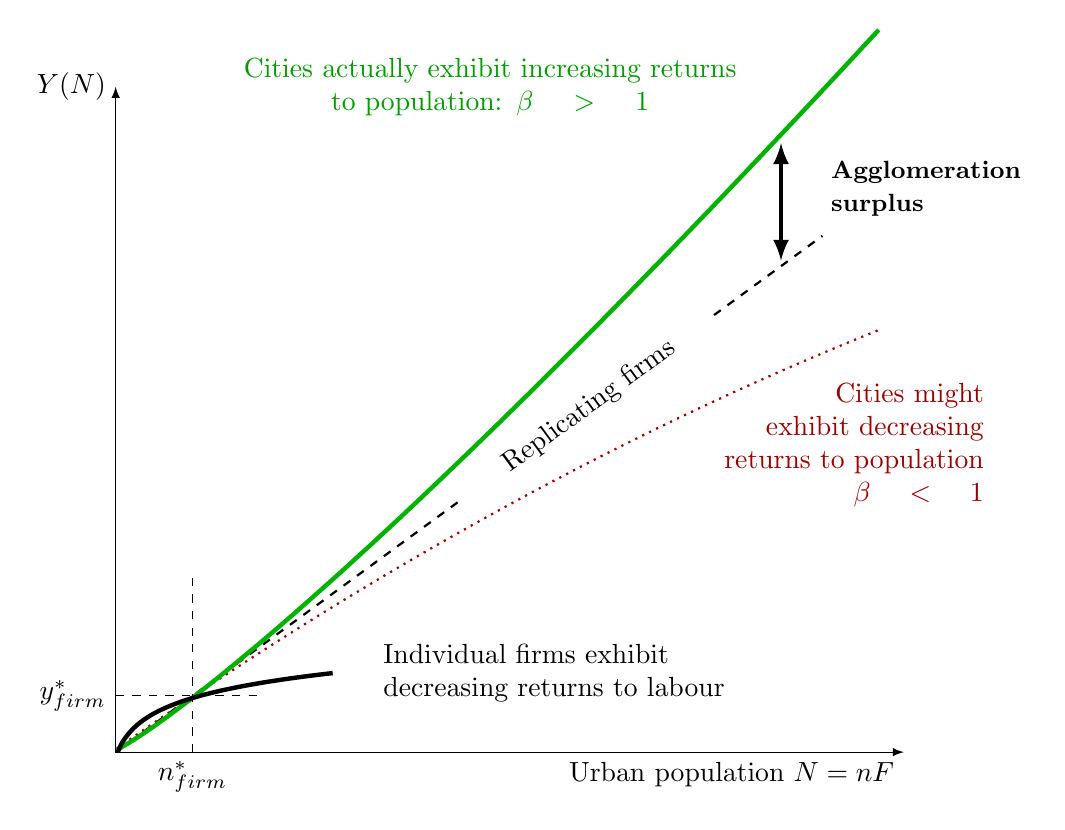
\begin{tikzpicture}[scale=.65, my plot/.style={thick, smooth, samples=100, domain=0.1:2.2},
plot2/.style={thick, smooth, samples=100, domain=0.1:14.99},
                    my grid/.style={dashed,opacity=0.5, every node/.style={black,opacity=1}},
                    my axis/.style={latex-latex}]
 
 \draw[my axis] (0,13)node[left] {$Y(N)$} --(0,0)-- (15.4, 0) node[below left] {Urban population $N=nF$}; %creates the axis
 % \node at (0,13)[below left]{y(n)};

\coordinate (origin) at (0,0);
\def\x{0.45}
\def\y{2.1}
\def\b {$15/(2*ln(\y)+.05)$};
%\def\p{0.55} % define the x, y and p )(midpointvalues
%\draw[my plot] (0,0) plot (\x,{ln(\x)});  %Draws curve
%\draw[my plot] (0,0) plot ({\x-.08},{2.3+ln(\x)}); 
\coordinate (Uy) at (\y,{2*ln(\y)+.05});

% THREE SCALE POSSIBILITIES:LINES
%\draw [thick, dashed](0,0)--(14, 10.22583);%node[below right, text width=1.5cm]{replicating firms};%{$\frac{N}{n_R}y_R$};   %diagonal line CRS


\node at (7, 10.22583*7/14) (nodeA) {};
\node at (11.5, 10.22583*11.5/14) (nodeB) {};
\node at (14, 10.22583) (nodeC) {};

\draw [thick, dashed](0,0) -- (nodeA);
\draw [thick, dashed](nodeB) -- (nodeC);
\draw [thick, dashed, opacity=0] (nodeA) -- (nodeB) node [midway,  sloped, opacity=1] (TextNode) {Replicating firms};
%\draw [decoration={text along path,
    % text={replicating firms},text align={right}},decorate]  (nodeA) -- (nodeB);

   

\draw[plot2, dotted, red!60!black, ] (0,0) plot ({\x-.08},{(.7*\x)-(\x/10)^2 });%{(\x)^0.9/1.5 }); %DRS
\node at (13.5,6)[text width=4.5cm, align=right, red!60!black,opacity=50] 
    {Cities might\\ exhibit decreasing \\returns to population \\ $\beta<1$};% DRS
    
\draw[plot2, ultra thick, green!70!black] (0,0) plot ({\x-.08},{(\x/1.5)^1.15});%
\node at (15.2,13) [left, text width=10cm, green!60!black, align=center ]{ Cities actually exhibit increasing returns\\ to population: $\beta>1$};%IRS
% \node at (15.4, 13.5){$AN^\beta$};
%\draw[plot2, red, thick, dashed, opacity=.5] (0,0) plot ({\x-.08},{(\x/1.5)^1.15+.2});%
% ARROW
\draw[latex-latex, ultra thick] (13, 11.9)--(13, 9.6);
\node at (15.9, 11.)[ text width=2.5cm, align=left]
    {\small\textbf{Agglomeration\\ surplus}};

\begin{scope}[ yscale=1,xscale=2]% shift={(1.9,0)} 
	\coordinate (Uy) at (\y, {2.3+ln(\y)});
  \draw[my plot,ultra thick] (0,0) plot ({\x-.08},{1.15+ln(\x)/2})
    node[right=.5cm, text width=7cm]{Individual firms exhibit \\decreasing returns to labour}; % production function for generic ferm
\draw[dashed](.75, 0)node[below]{$n_{firm}^*$} --(.75, 3.4);
 \draw[dashed](0,  1.1)node[left]{$y_{firm}^*$} --(1.4,  1.1);
\end{scope}
\end{tikzpicture}